\documentclass[report]{subfiles}

\begin{document}
\label{sec:result}
The following section contains the results of the implementation section.

\subsection{KNN}
\label{sec:resultKNN}
The result of the easy problem with KNN can be seen at figure~\ref{fig:knnEasyProblem}. The setting with 'sigma = 1' in smoothing and 0.99 principle components gives a success of approx 86\% with k as 1. The algorithm was also tested with K-Means, but initial testing shown that the time to compute the k-means was too significant and the end result was a lot lower than with PCA, also if done in combination with PCA.\\
One thing to note is that there are not a big difference with the k-values, they are however slowly dropping in success the higher a k-value.

\begin{figure}[H]
	\centering
	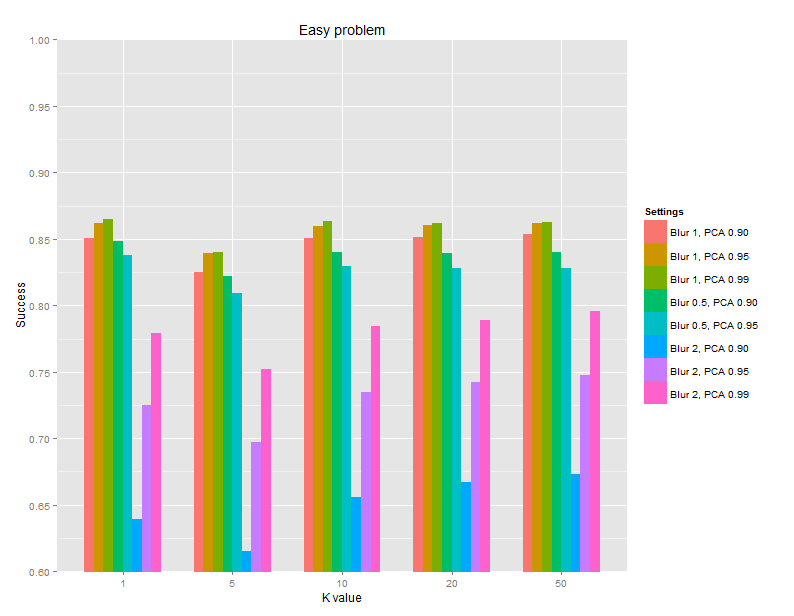
\includegraphics[width=1\textwidth]{images/knnEasyProblem}
	\caption{Figure of the result after running KNN on the easy problem}
	\label{fig:knnEasyProblem}
\end{figure}

The best settings from the easy problem was then used with the hard problem, and the results can be seen at figure~\ref{fig:knnHardProblem}, where the best hand writing is at approx 84\% success and the worst is at approx 42\%. Running with different k-values and PCA percentages did not change much, it was still the same two people low in the success and the same two to three with the highest success.

\begin{figure}[H]
	\centering
	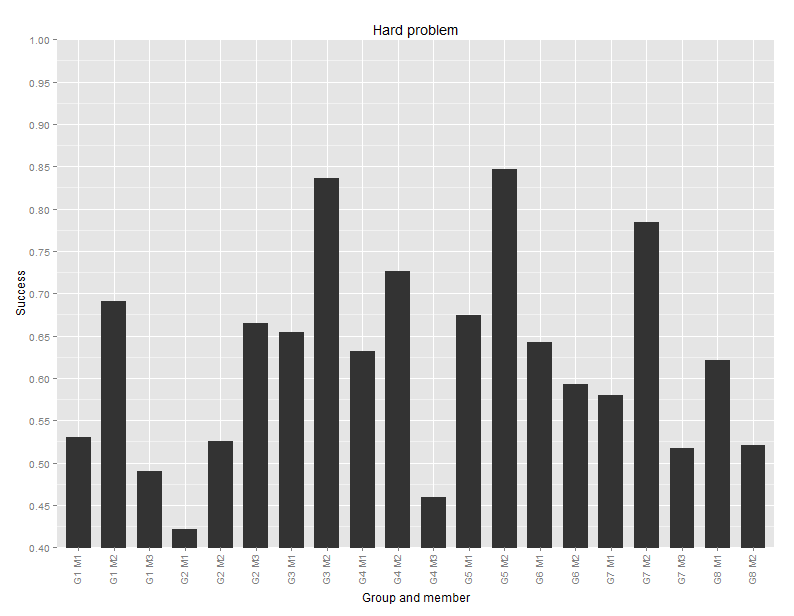
\includegraphics[width=1\textwidth]{images/knnHardProblem}
	\caption{Figure of the result after running KNN on the hard problem}
	\label{fig:knnHardProblem}
\end{figure}

\subsection{Random Forest}
\label{sec:resultRandomForest}

\subsection{Who has the worst hand writing?}


\end{document}